\section{Bundle Protocol and Security Specifications}
\label{sec:dtn}

The delay Tolerant Architecture defines a network architecture for irregularly connected networks subject to frequent partition and possibly long propagation delays \cite{cerf2007delay}. To face these particular properties, the authors proposed an overlay layer, called the \textbf{bundle layer}, which provides end-to-end reliable messages delivery. This layer works over the transport, network or data link layer using different convergence layer to communicate with lower layer protocols. The Bundle protocol specification \cite{rfc5050} defines the services offered by the bundle layer, bundle format, bundle processing and convergence layers. 

\begin{figure}[ht]
\centering
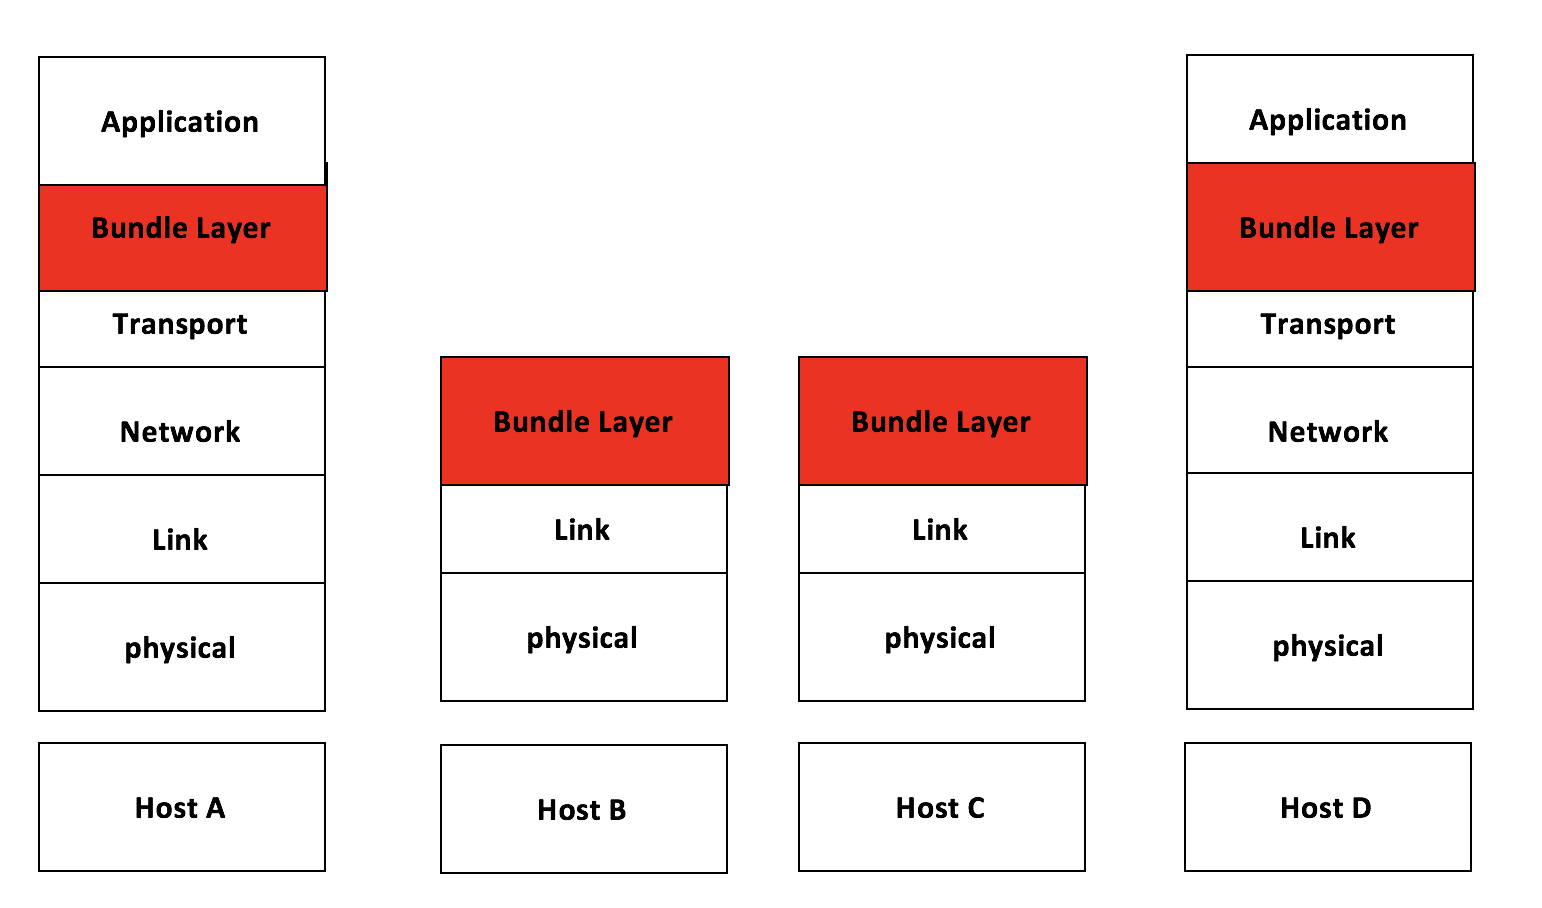
\includegraphics[width=1 \linewidth, height=9.5cm]{images/bundle.png} 
\caption{Bundle layer}
\label{fig:bundle}
\end{figure}

A bundle is the basic data unit of the Bundle protocol, similar to a packet for the IP protocol. A \textbf{bundle node}, DTN node or just simply a node could be any entity that can send or receive bundles, in other words, it is an implementation of the bundle layer. Note that a spacecraft could contain more than one instance of the Bundle protocol. For instance, the International Space Station is considered a network itself rather than a single bundle node. Negotiation between nodes might not be possible due to the delay and disruption, so a bundle is a self-contained data structure which has enough processing information.


The bundle layer provides persistent storage, hop-by-hop transfer, late binding, and optional end-to-end acknowledgement to overcome the constrained environment. The Bundle Protocol employs Universal Resources Identifiers URI as naming scheme, this flexible model allows the encapsulation of different addressing schemes and late binding. 

According to CCSDS \cite{rationale2010requirements}, the Bundle protocol is the best-suited option to support in-space internetworking. There is ongoing work within the CCSDS to adapt and standardise the Bundle protocol and the security specifications. %The next section describes the security specification for the Bundle protocol. 

Many successful experiments of the Bundle protocol were already performed in deep space. The first experiment was conducted by Surrey Satellite Technology back in 2008. The test consisted on deliver images taken by the UK-DMC Disaster Monitoring Constellation satellites to ground stations using the Bundle Protocol \cite{ivancic2010experience}. NASA employed the Bundle protocol in the Deep Impact Space Network experiment for around four weeks. There is a pilot operation on the International Space Station for many years as well. \cite{araniti2015contact}.    


%\subsection{Security for DTN in space}


 %From the beginning, the Delay-Tolerant Research Group worked on the security specifications for the Bundle protocol. The motivation was to provide data integrity and confidentiality services to the bundle layer. As space missions are more connected to the Internet and the economic value of space assets are very high is comprehensible consider information security as a critical component of the communication system.
 
 
 The Bundle Security Protocol \cite{rfc6257} provides the specifications for data integrity and confidentiality services to the Bundle protocol. The document defines the data structure to provide the security services as extension blocks. A new document, still in active development \cite{ietf-dtn-bpsec-07}, defines two types of security blocks: Block Integrity Block (BIB) and Block Confidentiality Block (BCB). Previous versions of the specification define an extra security block, the Block Authentication Block BAB which was intended to provide hop-by-hop authentication but was removed in the last version of the document.     
 
 
 Section of a space-based DTN may be untrusted, requiring traditional security services. However, stressed environment, already mentioned in this report, impose conditions where traditional mechanisms are not adequate. Access to a certificate authority cannot be assumed, interactive protocols are unlikely to be successful and consumption of scarce resources cannot be allowed.
 
 
 The Bundle protocol allows a mix of ``security-aware'' nodes and ``non-security-aware'' nodes within the same network. For space-based networks, the lack of physical resources or security being implemented in other layers are potential scenarios for this situation. A space DTN operates as an overlay network on the top of lower layers. Thus, the first threat is non-DTN nodes which could exploit vulnerabilities in the bundle layer \cite{rfc6257}.
 
Scarce resources make unauthorised access a major problem for a space DTN, especially in the space segment. Denial of service (DoS) attack is another concern for DTNs in space. Even worse, attackers could take advantage of long delays to make DoS attacks more effective \cite{rfc6257}. 

 
%\subsection{Key Management for DTN in space}
In a multi-hop communication, intermediate security-aware nodes may verify the integrity of the bundles or decrypt them according the security specifications. Security-aware-nodes thus may need the corresponding verification or decryption keys. This requirement implies that any key management solution must consider this situation to meet the security specification.

There is always a trade-off between usability against security. Security adds overhead, but the limited resources of some DTN nodes in the space segment requires to keep bandwidth and storage overhead low. Otherwise, mission planners will reject the security implementation. \cite{book2012architecture}.


%The next section is a literature review of the so far proposed key management solutions for DTN in space.



BSP is built on the assumption that DTN nodes already have access to authenticted copies of other's public keys.







